%
% main.tex -- Paper zum Thema wwt
%
% (c) 2019 Michael Schmid, Hochschule Rapperswil
%
\chapter{Wetter-Wavelet-Transformation\label{chapter:wwt}}
\lhead{Wetter-Wavelet-Transformation}
\begin{refsection}
\chapterauthor{Michael Schmid}



\definecolor{codegreen}{rgb}{0,0.6,0}
\definecolor{codegray}{rgb}{0.5,0.5,0.5}
\definecolor{codepurple}{rgb}{0.58,0,0.82}
\definecolor{backcolour}{rgb}{0.95,0.95,0.92}

\lstdefinestyle{mystyle}{
	backgroundcolor=\color{backcolour},   
	commentstyle=\color{codegreen},
	keywordstyle=\color{magenta},
	numberstyle=\tiny\color{codegray},
	stringstyle=\color{codepurple},
	basicstyle=\footnotesize,
	breakatwhitespace=false,         
	breaklines=true,                 
	captionpos=b,                    
	keepspaces=true,                 
	numbers=left,                    
	numbersep=2pt,                  
	showspaces=false,                
	showstringspaces=false,
	showtabs=false,                  
	tabsize=2
}
\lstset{style=mystyle}
\lstdefinestyle{mystyle}{
	morekeywords={cwt,contourf,datetick}
}


\section{Einführung}
\rhead{Einführung}


Seit langen konsultiere ich meine aktuellen Wetterdaten von eher unüblichen Wetter Internetseite.
Dabei handelt es sich um eine Privat geführte Wetterstation welche die gemessenen Daten, kostenlos und sehr rudimentär im Internet grafisch darstellt und auch tabellarisch zur Verfügung stellt.
Das Feature welches is bis anhin regelmässig nutze, war die grafische Darstellung der aktuellen Wetterdaten über den Zeitraum der letzten 24 Stunden.
Bei speziellen Ereignissen des Wetters vielen mir besondere und regelmässige Charakteristiken auf.
\\
\\
Nach der Einführung in die Theorie der Wavelets kam mir die Idee solche Wetterphänomene mittels einer geeigneten Wavelet Transformation zu detektieren.
In diesem Paper wird einerseits auf die theoretische Grundlage der Angewendeten Methoden sowie den besprochenen meteorologischen Phänomene zurückgegriffen und kurz erläutert. 
Weiter wird auf den Prozess der eigentlichen Inhaltes des Papers vertieft eingegangen. Ein besonderes Augenmerk wird auf die allgemeine Vorgehensweise sowie deren Schwierigkeiten gelegt.
\\




\section{Wetterstation Seegräben}
\rhead{Wetterstation Seegräben}

Die Wetterstation Seegräben ist eine privat geführte Wetterstation in der Gemeinde Seegräben im Kanton Zürich.

Die Wetterstation ist aus einer DAVIS Vantage Pro2 6153 aufgebaut.
Diese besteht aus einem Thermo- und  Hydrosensor, einem Windgeschwindigkeit und Richtungsmesser sowie einem Regenmesser. 
Durch diese Sensoren werden folgende Daten aufgezeichnet:
\\
\\
\\

\begin{minipage}{0.5\textwidth}
\begin{itemize}
	\item Aussentemperatur
	\item Luftfeuchtigkeit
	\item Luftdruck
	\item Windgeschwindigkeit

\end{itemize}	
\end{minipage}
\begin{minipage}{0.5\textwidth}
\begin{itemize}
	\item Windböen
	\item Windrichtung
	\item Regenmenge
	\\
	\\
\end{itemize}	
\end{minipage}
\\
\\

Der Thermo- / Hydrosensor liegt zusammen mit dem Regenmengenmesser auf 2 Meter über dem Boden. Mit einem Abstand von rund 10 Meter zum nächsten Gebäude, werden optimale Messbedingungen geschaffen. Der Windmesser wurde am First des Gebäudes montiert. Mit einem Masten werden die Daten 1,5 Meter über dem First gemessen 

Die Daten werden anschliessend mit einer Software von PC-Wetterstation.de weiterverarbeitet und auf eine rudiment\"aren Website Dargestellt. Mehr zur Verwendung der Wetterdaten im n\"achsten Kapitel




\section{Datenaufarbeitung}
\rhead{Datenaufarbeitung}
\subsection{Wetter-Archiv}
Als n\"achster Schritt der Vorbereitung zur Wavelet Transformation, war die Aufbereitung der zur Verf\"ugung gestellten Daten der Wetterstation Seegr\"aben.
Dazu musste erst analysiert werden wie die Daten auf der Website dargestellt werden.
In der Sektion des Archiv auf der Website kann man die Wetterdaten im gew\"unschten Zeitraum tabellarisch darstellen lassen.
\subsection{Datenerfassung}
Da f\"ur meine Anwendung eine M\"oglichst genaue Aufl\"osung der jeweiligen Daten erforderlich ist, mussten die Daten im Zeitraum von einem Tag dargestellt werden. 
Dies hatte zur Folge, dass man f\"ur jeden Tag ein Tabelle auf dem Archiv der Website \"offnen musste. 
Da mir die Zeit sowie auch die Lust fehlte jeden einzelnen Tag separat zu \"offnen und die Daten mittels "Copy und Paste" Verfahren in eine Excel-Tabelle einzuf\"ugen, War die Motivation gross  ein Programm zu schreiben welche diese Aufgabe automatisieren sollte.
Als Programmiersprache wurde hierf\"ur Python gewählt.
Wie es so üblich ist mit Python, hat man das Wissen für zur Vollendung der Aufgabe nicht sogleich auswendig präsent, doch dank kurzen und gezielten Goolge abfragen sowie Besuchen des Stackoverflow Forums konnte das Wissen schnell angeeignet werden.
Mit der Pandas Library und der Funktion "read\_html"\space konnten die Daten direkt mittel Aufruf aus dem Python Programm von der URL-Seite heruntergeladen werden.
Entscheidend für das Gelingen dieser Teilaufgabe war, dass die URL-Links der einzelnen Tage jeweils regelmässig aufgebaut sind.
Da dies der Fall war, konnten die entsprechenden Link mittels einer einfachen While-Schleife zusammengesetzt werden.
\newpage
Folgend der essenzielle Ausschnitt aus dem Python Code:

\begin{figure}[h]
	\centering
	\lstinputlisting[language=Python,firstline=1,lastline=16,numbers=left,style = mystyle]{/home/nunigan/Documents/MathSem/SeminarWavelets/buch/papers/wwt/pictures/get_data.py}
	\caption{Python Codeausschnitt}
	\label{fig:python-code}
\end{figure}

Die Daten konnten als nächster Schritt in einer Excel-Tabelle abgespeichert werden.
Dort folgte der letzte feinschliff, dabei wurden alles überflüssigen Kopfzeilen und Statistiken entfernt.

\subsubsection{Unregelmässigkeiten der Wetterstation}
Bei der Datenerfassung durch das eben beschriebene Python Programm wurden einige Unregelmässigkeiten er Wetterstation Seegräben festgestellt.
Das Programm wird jeweils durch einen Fehler abgebrochen, wenn der angegebene Link nicht abrufbar ist. 
So fiel mir auf, dass unregelmässig auf das Jahr verteilt, gewisse Daten von Tagen fehlen, sprich der Link ist nicht abrufbar.
Wenn man manuell auf der Website nach diesem Tag sucht, wird man auch nicht fündig.
Dies trat teilweise sogar in Abschnitten von mehreren Tagen auf.
Wie sich später herausstellte traten die fehlenden Tagen nicht zu den Zeitpunkten auf welche mich interessierten.
\newpage

\subsection{Datendarstellung}
Die Darstellung der gewonnen Daten konnten einfach mittels Matlab gemacht werden. Anbei die Plot der Rohdaten aus dem Jahre 2018, wobei nur jeder 10 Messpunkt geplotet wurde. Diese Rohdaten dienten als Grundlage für alle weiteren Berechnungen. 

\begin{figure}[h]
\centering
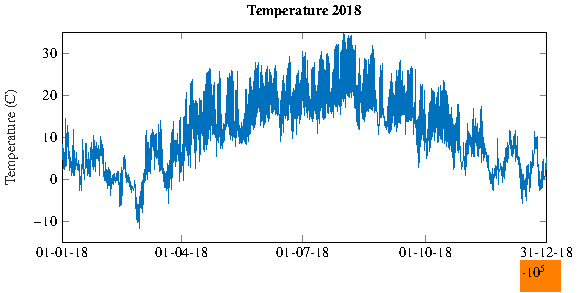
\includegraphics[width=0.9\textwidth]{papers/wwt/images/raw_temp_wwt.pdf}
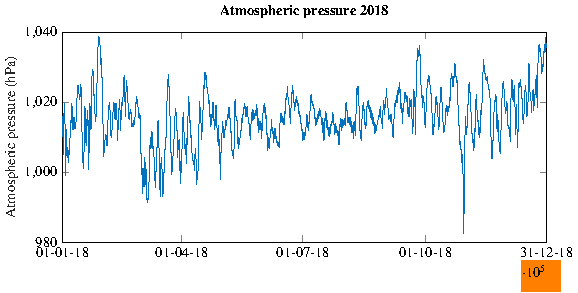
\includegraphics[width=0.9\textwidth]{papers/wwt/images/raw_airp_wwt.pdf}
\caption{Rohdaten Temperatur und Luftdruck 2018}
\end{figure}


\begin{figure}[h]
	\centering
	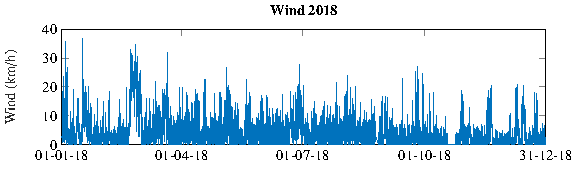
\includegraphics[width=0.9\textwidth]{papers/wwt/images/raw_wind_wwt.pdf}
	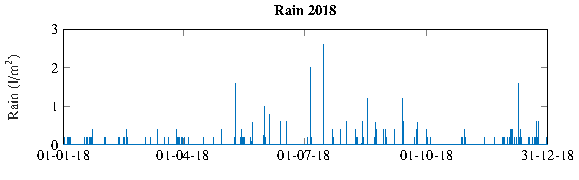
\includegraphics[width=0.9\textwidth]{papers/wwt/images/raw_rain_wwt.pdf}
	\caption{Rohdaten Wind und Regen2018}
\end{figure}

\newpage
\newpage

töliwjfölsfs
fds
f
dsfdsf

\section{Stetige Wavelet-Transformation}
\rhead{Stetige Wavelet-Transformation}

Die Theoretischen Grundlagen rund um die Stetige Wavelet-Transformation wurde im Kapitel 4 genaustens erläutert. 
In diesem Abschnitt der Seminararbeit wird öfters auf die Theorie des angesprochene Kapitel 4 referenziert ohne diese weiter zu erläutern. 
Für die genaue Untersuchung vom Signalen, wobei möglichst viele Information gewonnen werden sollten, eignet sich die Stetige Wavelet-Transformation (folgend noch kurz cwt, aus dem Englishen continuous wavelet transform)
ideal. 
Regelmässig auftretende Frequenzen können dank der cwt gefunden und zusätzlich auch einem Zeitraum zugeteilt werden.


\section{Analyse von Wettereignissen}
\rhead{Analyse von Wetterereignissen}

\subsection{Sturmtief}
\rhead{Sturmtief}


\section{Schlussfolgerung}
\rhead{Schlussfolgerung}

\printbibliography[heading=subbibliography]
\end{refsection}
